% KU Leuven latex poster template
%
% © 2015 Michael Hofmann
%
% This work is licensed under the Creative Commons Attribution 3.0 Unported License.
% To view a copy of this license, visit
% http://creativecommons.org/licenses/by/3.0/ or send a letter to Creative
% Commons, 444 Castro Street, Suite 900, Mountain View, California, 94041, USA.

\documentclass[english,xcolor=table,t
]{beamer}

\usepackage[size=custom,width=100,height=100
    ,width=90,height=140,scale=1.2
]{tex/beamerposter}

\usepackage[utf8]{inputenc}
\usepackage[T1]{fontenc}
\usepackage{amsmath}
\usepackage[nolist,nohyperlinks]{acronym}
\usepackage{babel,lmodern,graphicx,mathptmx,xspace,wasysym,microtype,booktabs,tabularx,relsize,textcomp,longtable,lipsum,colortbl,eurosym,url,multicol,etoolbox,multimedia,pdfpages,fixltx2e,ifluatex,epstopdf}
\usepackage[olditem,oldenum]{paralist}
\usepackage[babel=true]{csquotes}
\usepackage[thinqspace,amssymb,textstyle]{SIunits}
\usepackage[textsize=tiny]{todonotes}
\usepackage[symbol]{footmisc}
\usepackage[notquote]{hanging}
\usepackage[normalem]{ulem}

\pdfstringdefDisableCommands{\renewcommand{\sout}{}}
\graphicspath{{figures/}}
% Fix sort order in case the same file exists with multiple extensions
\DeclareGraphicsExtensions{.pdf,.png,.jpeg,.jpg,.eps}
\frenchspacing

\ifluatex\else
% textcomp defines 00B1 wrong, so fix it here
\DeclareUnicodeCharacter{2192}{\ensuremath{\rightarrow}}
\DeclareUnicodeCharacter{2194}{\ensuremath{\leftrightarrow}}
\DeclareUnicodeCharacter{2212}{\ensuremath{-}}
\DeclareUnicodeCharacter{22EE}{\ensuremath{\vdots}}
\DeclareUnicodeCharacter{22EF}{\ensuremath{\cdots}}
\DeclareUnicodeCharacter{00B1}{\ensuremath{\pm}}
\DeclareUnicodeCharacter{00D7}{\ensuremath{\times}}
\DeclareUnicodeCharacter{221E}{\ensuremath{\infty}}
\DeclareUnicodeCharacter{2248}{\ensuremath{\approx}}
\DeclareUnicodeCharacter{2264}{\ensuremath{\leq}}
\DeclareUnicodeCharacter{2265}{\ensuremath{\geq}}
\DeclareUnicodeCharacter{03BC}{\micro}
\DeclareUnicodeCharacter{2206}{\ensuremath{\Delta}}
\fi

\newcommand{\m}[1]{\todo[noline,bordercolor=orange!20,backgroundcolor=orange!20]{#1}}

\newcommand{\eg}{e.\,g.\xspace}
\newcommand{\ie}{i.\,e.\xspace}

\addunit{\octave}{octave}
\addunit{\pbdrunit}{\%BDR}
\addunit{\plbdrunit}{\%LBDR}
\addunit{\currentunit}{cu}
\addunit{\pulsespersecondunit}{pps}

\newcommand{\pps}[1]{\unit{#1}{\pulsespersecondunit}}
\newcommand{\hz}[1]{\unit{#1}{\hertz}}
\newcommand{\khz}[1]{\unit{#1}{\kilo\hertz}}
\newcommand{\mhz}[1]{\unit{#1}{\mega\hertz}}
\newcommand{\db}[1]{\unit{#1}{\deci\bel}}
\newcommand{\us}[1]{\unit{#1}{\micro\second}}
\newcommand{\ms}[1]{\unit{#1}{\milli\second}}
\newcommand{\s}[1]{\unit{#1}{\second}}
\newcommand{\pc}[1]{\unit{#1}{\%}}
\newcommand{\pmil}[1]{\unit{#1}{\permil}}
\newcommand{\pcdb}[1]{\unit{#1}{\%\per\deci\bel}}
\newcommand{\de}[1]{\unit{#1}{\degree}}
\newcommand{\uv}[1]{\unit{#1}{\micro\volt}}
\newcommand{\nv}[1]{\unit{#1}{\nano\volt}}
\newcommand{\bdr}[1]{\unit{#1}{\pbdrunit}}
\newcommand{\lbdr}[1]{\unit{#1}{\plbdrunit}}
\newcommand{\cu}[1]{\unit{#1}{\currentunit}}
\newcommand{\nhl}[1]{\unit{#1}{\deci\bel{}\textnormal{nHL}}}
\newcommand{\hl}[1]{\unit{#1}{\deci\bel{}\textnormal{HL}}}
\newcommand{\spl}[1]{\unit{#1}{\deci\bel{}\textnormal{SPL}}}
\newcommand{\spla}[1]{\unit{#1}{\deci\bel{}\textnormal{SPL(A)}}}
\newcommand{\dbfs}[1]{\unit{#1}{\deci\bel{}\textnormal{FS}}}
\newcommand{\pespl}[1]{\unit{#1}{\deci\bel{}\textnormal{peSPL}}}
\newcommand{\pespla}[1]{\unit{#1}{\deci\bel{}\textnormal{peSPL(A)}}}
\newcommand{\sd}[1]{\ensuremath{\textnormal{SD}=#1}}
\newcommand{\se}[1]{\ensuremath{\textnormal{SE}=#1}}
\newcommand{\ir}[1]{\ensuremath{\textnormal{IR}=#1}}
\newcommand{\el}[2]{\ensuremath{\textnormal{#1}_{\textnormal{#2}}}}

% pandoc >=1.14
\providecommand{\tightlist}{\setlength{\itemsep}{0pt}\setlength{\parskip}{0pt}}


\usepackage[style=authoryear-comp,natbib=true,backend=bibtex]{biblatex}
\ExecuteBibliographyOptions{
    bibencoding=ascii,
    texencoding=utf8,
    backref=false,
    dashed=false,                                    % no dash instead of recurring author and editor names
    maxnames=2,
    maxbibnames=99,
    uniquename=init,firstinits=true,terseinits=true, % only care about initials
    useprefix=true,                                  % sort van Wieringen correctly
    sortcites=false,                                 % do not sort multiple citations
    doi=false,
    url=false,
}
\AtEveryBibitem{\clearfield{month}}
\DeclareFieldFormat{eprint:pubmed}{\iffootnote{}{\mkbibacro{PMID}\addcolon\space
  \ifhyperref
    {\href{http://www.ncbi.nlm.nih.gov/pubmed/#1}{\nolinkurl{#1}}}
    {\nolinkurl{#1}}}}
\DeclareFieldFormat{isbn}{\iffootnote{}{\mkbibacro{ISBN}\addcolon\space
  \ifhyperref{\href{http://amzn.com/#1}{\nolinkurl{#1}}}{\nolinkurl{#1}}}}
\DeclareFieldFormat{issn}{}
\setlength\bibhang{2em}

\addbibresource{bib/bib.bib}

% beamer
\mode<presentation>

\newbox{\layoutbox}
\newlength{\headerheight}
\setlength\headerheight{18cm}
%\newlength{\logowidth}
\setlength\logowidth{\headerheight*\ratio{236px}{661px}}
\setlength\logowidth{\headerheight}

\definecolor{kuldark}{HTML}{123C75}   % heading background
\definecolor{kulbgleft}{HTML}{CBE1EC} % background fill gradient left
\definecolor{kulbgright}{HTML}{C5D9E4} % background fill gradient right
\definecolor{kulheaderleft}{HTML}{158DB0} % header fill gradient left
\definecolor{kulheaderright}{HTML}{03708D} % header fill gradient right

% headline colors and fonts
\setbeamercolor{headline}{fg=white}
% large, Large, LARGE, huge, Huge, veryHuge, VeryHuge, VERYHuge
\setbeamerfont{title in headline}{size=\huge,series=\bfseries}
\setbeamerfont{author in headline}{size=\LARGE}
\setbeamerfont{institute in headline}{size=\LARGE}

% footline colors and fonts
\setbeamercolor{footline}{fg=white}
\setbeamerfont{footline}{size=\normalsize}

% body colors, and fonts
\setbeamercolor*{normal text}{fg=black}
\setbeamerfont*{block body}{size=\Large}

% block environment
\setbeamercolor*{block body}{bg=white,fg=black}
\setbeamercolor*{block title}{fg=white,bg=kuldark}
\setbeamerfont{block title}{size=\Large,series=\bfseries}

\setbeamercolor{structure}{fg=kuldark}
\setbeamerfont{structure}{size=\large}
\setbeamerfont*{item}{parent=\large}
\setbeamerfont{caption}{}

\setbeamertemplate{background canvas}{%
  \pgfdeclarehorizontalshading{backgroundshading}{\the\paperheight}{color(0cm)=(kulbgleft); color(\the\paperwidth)=(kulbgright)}%
  \setbox\layoutbox=\hbox{\pgfuseshading{backgroundshading}}%
  \setbox\layoutbox=\hbox{\lower\paperheight\hbox{\box\layoutbox}}%
  \wd\layoutbox=0pt\ht\layoutbox=0pt\dp\layoutbox=0pt%
  \box\layoutbox%
  \leavevmode
  \begin{beamercolorbox}[ht=1ex,wd=\paperwidth]{headline}%
    \begin{columns}[T,totalwidth=\paperwidth]
      \begin{column}{\paperwidth}
        \vskip\paperheight
        \vskip-50cm
		      \end{column}
    \end{columns}
  \end{beamercolorbox}
}

% no navigation on a poster
\setbeamertemplate{navigation symbols}{}

\setbeamertemplate{headline}{%
  \pgfdeclarehorizontalshading{headlineshading}{\headerheight}{color(0cm)=(kulheaderleft); color(.3*\the\paperwidth)=(kulheaderleft); color(\the\paperwidth)=(kulheaderright)}%
  \setbox\layoutbox=\hbox{\pgfuseshading{headlineshading}}%
  \setbox\layoutbox=\hbox{\lower\headerheight\hbox{\box\layoutbox}}%
  \wd\layoutbox=0pt\ht\layoutbox=0pt\dp\layoutbox=0pt%
  \box\layoutbox%
  \leavevmode
  \begin{beamercolorbox}[ht=1ex,wd=\paperwidth]{headline}%
    \begin{columns}[T,totalwidth=\paperwidth]
      \begin{column}{2cm}
      \end{column}
      \begin{column}{\paperwidth-4cm-\logowidth}
        % Change the size and the line skips to fit in the title bar
        \vskip2cm
        {\usebeamerfont{title in headline}\inserttitle\\[.5ex]}
        {\usebeamerfont{author in headline}\insertauthor\\[1ex]}
        {\usebeamerfont{institute in headline}\insertinstitute}
      \end{column}
      \begin{column}{2cm}
      \end{column}
      \begin{column}{\logowidth}
%        \raggedleft
\includegraphics[width=\headerheight,angle=-90]{images/lg.png}
        \raggedleft
\includegraphics[height=\headerheight]{images/lg.png}
      \end{column}
    \end{columns}
  \end{beamercolorbox}
  \vskip-1em
  \vskip-1cm
}

\setbeamertemplate{footline}{
  \pgfdeclarehorizontalshading{headlineshading}{4ex}{color(0cm)=(kulheaderleft); color(.3*\the\paperwidth)=(kulheaderright); color(\the\paperwidth)=(kulheaderright)}%
  \setbox\layoutbox=\hbox{\pgfuseshading{headlineshading}}%
  \setbox\layoutbox=\hbox{\lower4ex\hbox{\box\layoutbox}}%
  \wd\layoutbox=0pt\ht\layoutbox=0pt\dp\layoutbox=0pt%
  \box\layoutbox%
  \leavevmode%
  \begin{beamercolorbox}[ht=4ex,leftskip=1cm,rightskip=1cm]{footline}%
    \url{winterwang.github.io} \hfill Aichi Medical University \hfill \texttt{abelardccwang@gmail.com}
    \vskip.8ex
  \end{beamercolorbox}
}

\setbeamertemplate{block begin}{%
  \vskip1cm%
  \begin{beamercolorbox}[ht=2.7ex,dp=0.9ex,rounded=false,shadow=false,leftskip=1cm]{block title}%
    \usebeamerfont*{block title}\insertblocktitle
  \end{beamercolorbox}%
  {\ifbeamercolorempty[bg]{block body}{}{\nointerlineskip\vskip-0.5pt}}%
  \usebeamerfont{block body}%
  \pgfsetfillopacity{.7}
  \advance\linewidth by -2cm
  \begin{beamercolorbox}[rounded=false,shadow=false,leftskip=0cm,sep=1cm,vmode,rightskip=0cm]{block body}%
    \ifbeamercolorempty[bg]{block body}{\vskip-.25ex}{\vskip-.75ex}\vbox{}%
    \parskip.4em
    \pgfsetfillopacity{1}
}

\setbeamertemplate{block end}{\end{beamercolorbox}}

\setbeamertemplate{structure text begin}{\vskip.4em}

\setbeamertemplate{itemize/enumerate body begin}{\begin{minipage}{\dimexpr\textwidth-2cm\relax}\vskip.4em}

\setbeamertemplate{itemize/enumerate body end}{\end{minipage}}

\setbeamertemplate{itemize items}[triangle]

\setbeamertemplate{bibliography item}{\hskip\dimexpr0.5em+0.8cm\relax}

\setbeamertemplate{caption}{%
  \parbox{\dimexpr\textwidth-2cm\relax}{%
  {%
    \usebeamercolor[fg]{caption name}%
    \usebeamerfont*{caption name}%
    \insertcaptionname~\insertcaptionnumber:%
  }
  \insertcaption\par
  }
}

\title{Changing trends in the prevalence of \emph{H. pylori} infection in Japan
(1908-2003): a systematic review and meta-regression analysis of 170,000
individuals}
\author{Chaochen Wang\textsuperscript{1}, Takeshi Nishiyama\textsuperscript{1},
Shogo Kikuchi\textsuperscript{1}, Manami Inoue\textsuperscript{2}, Norie
Sawada\textsuperscript{2}, Shoichiro Tsugane\textsuperscript{2},
Yingsong Lin\textsuperscript{1}}
\institute{1 Department of Public Health, Aichi Medical University, Nagakute,
Aichi, Japan;\\
2 Epidemiology and Prevention Group, Center for Public Health Sciences,
National Cancer Center, Tokyo, Japan}


\begin{document}


\begin{frame}

\begin{columns}

\column{(\linewidth-1cm)*\real{0.500000}}

\begin{block}{BACKGROUND}

\begin{itemize}
\item
  Gastric cancer burden remains high in Japan, where it is the
  second-leading cause of cancer deaths, accounting for annual deaths of
  approximately 50,000 in Japan.
\item
  Substantial evidence supports a central role for \emph{H. pylori} in
  the parthenogenesis of upper-gastrointestinal diseases, including
  peptic ulcer and noncardia gastric cancer.
\item
  Cross-sectional studies have suggested that the prevalence of \emph{H.
  pylori} infection increases with age, while the whole picture remains
  obscure.
\item
  We systematically reviewed the existing literature that presented
  estimates of the prevalence of \emph{H. pylori} infection in the
  Japanese population.
\item
  The obejectives are: (1) to derive a robust prevalence estimate of
  \emph{H. pylori} infection by birth year; (2) to clarify whether
  \emph{H. pylori} infection exhibits a birth-cohort pattern.
\end{itemize}

\end{block}

\begin{block}{Quick start}

Before starting, you have to install R, RStudio, bookdown package, and
other software and packages (\ie \texttt{Pandoc}, \LaTeX,
\texttt{rmarkdown}, \texttt{rticle}, \texttt{knitr}, etc.) which
bookdown depends on. See the official manual of
\href{https://bookdown.org/yihui/bookdown/}{bookdown} for details.

Installation:

\texttt{devtools::install\_github("pzhaonet/bookdownplus")}

Run the following codes, and you will get some files (e.g.~index.Rmd and
body.Rmd) and folders in your working directory.

\texttt{bookdownplus::bookdownplus()}

Now press \texttt{ctrl+shift+b} to compile it. Your will get a book file
named \texttt{index.pdf} in \texttt{\_book/} folder.

Write your own text in \texttt{index.Rmd} and \texttt{body.Rmd}, and
build your own lovely book. Have fun!

\end{block}

\begin{block}{Graphs}

Using \texttt{bookdown} or \texttt{rmarkdown}, users can insert figures
into a document in a friendly way. Just embed the R scripts into your
\texttt{.Rmd} file(s) and compile it/them with knitr package, and the
figures will appear automatically with high resolution and
reproductivity.

\begin{figure}
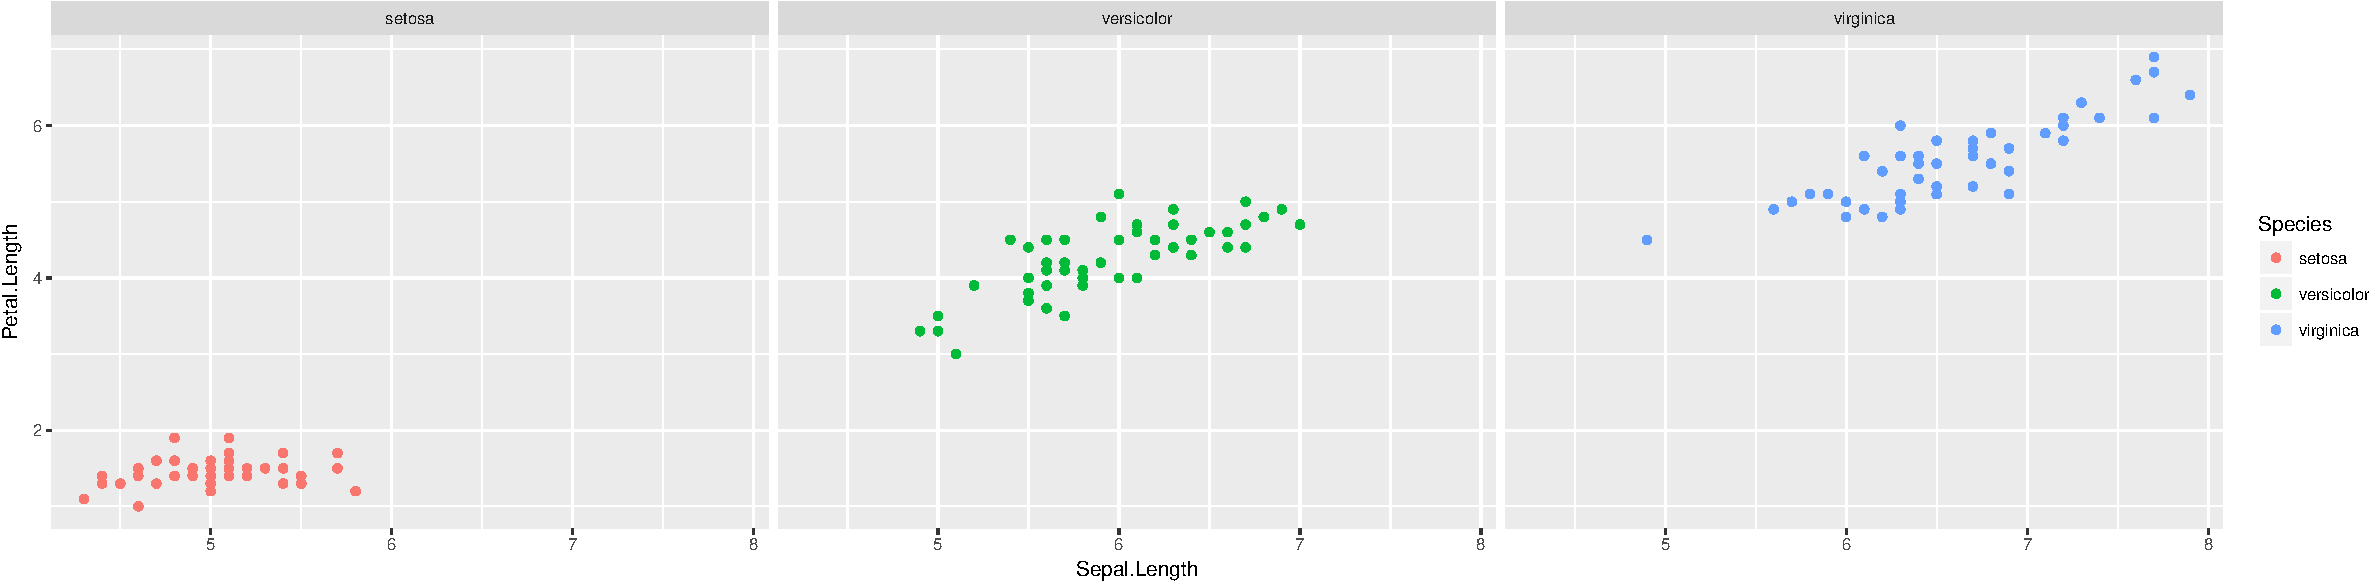
\includegraphics[]{poster-figures/iris-1.pdf}
\caption{IRIS data plotted with R ggplot2 package.}
\end{figure}

\end{block}

\begin{block}{Table}

Similarly to graphs, tables can be inserted either with R script or with
markdown syntax.

\begin{longtable}[]{@{}rrrrl@{}}
\toprule
Sepal.Length & Sepal.Width & Petal.Length & Petal.Width &
Species\tabularnewline
\midrule
\endhead
5.1 & 3.5 & 1.4 & 0.2 & setosa\tabularnewline
4.9 & 3.0 & 1.4 & 0.2 & setosa\tabularnewline
4.7 & 3.2 & 1.3 & 0.2 & setosa\tabularnewline
\bottomrule
\end{longtable}

\end{block}

\begin{block}{Bibliography}

\printbibliography

\end{block}

\column{(\linewidth-1cm)*\real{0.500000}}

\begin{block}{Book types supported by bookdownplus}

Some sample pages are displayed as follows. More details can be found in
the tutorial book \autocite{R-bdp}.

\begin{figure}[htp]
  
\includegraphics[width=.33\textwidth]{images/mail.pdf}\hfill
  
\includegraphics[width=.33\textwidth]{images/mail.pdf}\hfill
  
\includegraphics[width=.33\textwidth]{images/mail.pdf}
\end{figure}

\begin{figure}[htp]
  
\includegraphics[width=.33\textwidth]{images/mail.pdf}\hfill
  
\includegraphics[width=.33\textwidth]{images/mail.pdf}\hfill
  
\includegraphics[width=.33\textwidth]{images/mail.pdf}
\end{figure}

\begin{figure}[htp]
  
\includegraphics[width=.33\textwidth]{images/mail.pdf}\hfill
  
\includegraphics[width=.33\textwidth]{images/mail.pdf}\hfill
  
\includegraphics[width=.33\textwidth]{images/mail.pdf}
\end{figure}

\end{block}

\begin{block}{Take-home message}

\begin{itemize}
\item
  \texttt{R\ bookdownplus} is an extension of \texttt{bookdown} for
  academic and literal writing, especially for reproducible reports.
\item
  \texttt{R\ bookdownplus} is still being developed. Feel free to join
  me either in contributing templates to
  \href{https://github.com/pzhaonet/bookdownplus}{\textbf{my Github
  repo}} \footnote{https://github.com/pzhaonet/bookdownplus}, or in
  writing the tutorial of R bookdownplus \autocite{R-bdp}.
\end{itemize}

\end{block}

\begin{block}{Acknowledgements}

Many thanks to Dr.~Yihui Xie for his amazing generosity and incredible
patience in helping me get into the wonderful world of R bookdown.

The open source codes from Github and R community are much appreciated.

\vskip1.5cm

\end{block}

\end{columns}

\end{frame}


\end{document}
